 \item Generowanie zamówienia na dostawę części - scenariusz główny \\
 
 Opis słowny - ten przypadek użycia opisuje funkcjonalność generowania zamówienia na dostawę części, których ilość w magazynie spadnie poniżej zadanego poziomu, ustawianego oddzielnie dla każdej części. Jest to funkcjonalność bardzo ułatwiająca pracę pracownikom magazynu, którzy dbają o zaopatrzenie sklepu, ponieważ po ustawieniu minimalnej liczby sztuk towaru, system sam dba o to, żeby poziom ten zawsze był utrzymany, zwalniając z tego obowiązku pracowników. Skutkuje to także mniejszą liczbą pomyłek przy zamawianiu dostaw.
 
 \begin{longtable}{|p{5cm}|p{7cm}|}
 	\hline
	\textbf{Aktor} & Pracownik \\
	\hline
	\textbf{Warunki początkowe} & Posiadanie konta z uprawnieniami umożliwiającymi zarządzanie częściami, zalogowanie się do systemu \\
	\hline
	\textbf{Opis przebiegu interakcji} & Wybór opcji zarządzania dostawami na stronie głównej sklepu, wybranie opcji generowania zamówienia na dostawę, wprowadzenie danych, zatwierdzenie operacji \\
	\hline
	\textbf{Sytuacje wyjątkowe} & Brak \\
	\hline
	\textbf{Warunki końcowe} & Utworzenie dokumentu, zawierającego listę części które należy zamówić przy najbliższej dostawie \\
	\hline
 \end{longtable}
 
\begin{figure}[h!]
    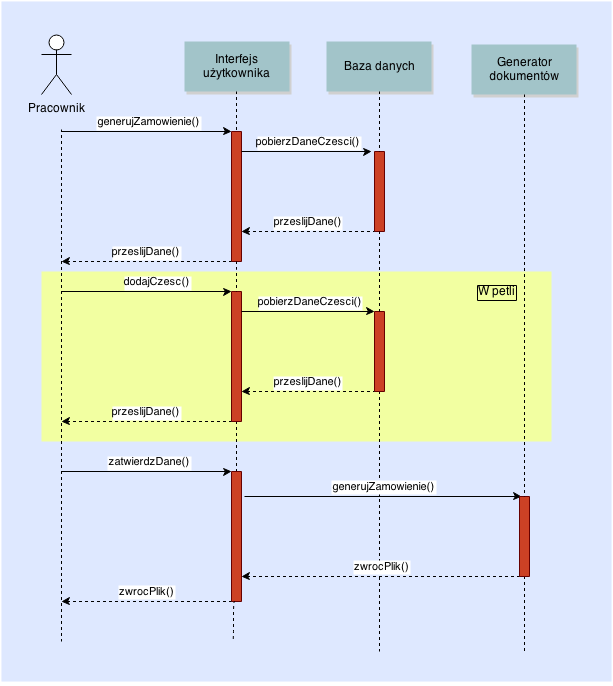
\includegraphics[width=\textwidth,
    height=0.7\textheight]{graphics/UseCase/Czesci/GenerowanieZamowieniaSD.png}
  \caption{Diagram sekwencji dla przypadku użycia Generowanie zamówienia na dostawę części - scenariusz główny}
\end{figure}
  \item Generowanie zamówienia na dostawę części - scenariusz główny \\
  \begin{tabularx}{\linewidth}{ c X}
  Aktor: & Pracownik \\
  \end{tabularx}
   \begin{enumerate}
    \item Pracownik otwiera stronę internetową sklepu, loguje się na swoje konto i wybiera opcję zarządzania dostawami.
    \item System prezentuje widok generowania zamówienia na dostawę, umożliwiający:
    \begin{enumerate}
      \item Dodanie typu części do zamówienia.
      \item Usunięcie wcześniej wprowadzonego typu części z zamówienia.
      \item Prezentację listy już wprowadzonych części.
    \end{enumerate}
    \item System początkowo wypełnia listę tymi częściami, których ilość w magazynie spadła poniżej zadanego minimalnego poziomu. Części dodawane są w minimalnej ilości wystarczającej do tego, aby poziom ten został osiągnięty.
    \item Pracownik dodaje nowe części według następującego schematu:
    \begin{enumerate}
      \item Pracownik wybiera przycisk umożliwiający dodanie typu części do zamówienia.
      \item System prezentuje listę części z możliwością wyszukiwania tak jak w przypadku użycia ``Wyświetlanie listy części''.
      \item Pracownik wybiera żądany typ części i wpisuje ilość sztuk (liczba naturalna większa od zera), jaka ma zostać dodana do zamówienia.
      \item Pracownik zatwierdza operację.
      \item Powrót do widoku generowania zamówienia.
    \end{enumerate}
    \item Po wprowadzeniu wszystkich informacji o zamówieniu, pracownik zatwierdza operację.
    \item System prosi pracownika o potwierdzenie zamiaru wygenerowania zamówienia.
    \item W przypadku potwierdzenia zamiaru przez pracownika, system generuje plik PDF z zamówieniem na dostawę.
    \item Pracownik pobiera plik i wysyła go do dostawcy.
  \end{enumerate}

